% math.tex — \input'd from thesis/experiments.tex
%
% Large-scale gradient ascent on sys for F=10 polytopes.
%
% Sources:
%   - Generated data: experiments/gradient-descent/gradient-descent.jsonl
%   - Plot script: experiments/gradient-descent/analyze.py
%   - Developer notes: experiments/gradient-descent/logbook.md
%   - Builds on: sec:sys-optimization (method, derivative formulae)
%   - Prose: agent-written, unreviewed
%
% Structure:
%   - Setup (brief, references sys-optimization)
%   - Results (table, scatter, headline finding)
%   - Convergence analysis (step-bound barrier — the key insight)
%   - Interpretation

\subsection{Large-Scale Gradient Ascent on sys}
\label{sec:gradient-descent}

Section~\ref{sec:sys-optimization} developed gradient ascent on
$\mathrm{sys} = c_{\mathrm{EHZ}}^2 / (2\,\mathrm{vol})$ and
demonstrated it on the polytopes from that section.
This section scales the procedure to ${\sim}1000$ starting polytopes,
all with $F = 10$, and distinguishes two structural classes.

\subsubsection*{Setup}

We generate two classes of random $F = 10$ polytopes:
\begin{enumerate}
\item \emph{General polytopes} ($N = 500$):
  normals uniform on~$S^3$, heights uniform in~$[0.8, 1.2]$.
  Capacity via the pruned HK2017 algorithm
  (Corollary~\ref{cor:adjacency-pruning}).

\item \emph{Lagrangian products} ($N = 501$, three buckets of~$167$):
  random polygon pairs $K_q \times_L K_p$ with facet splits
  $(F_q, F_p) \in \{(3,7),\,(4,6),\,(5,5)\}$.
  Capacity via the billiard algorithm
  (Theorem~\ref{thm:billiard-characterization}) with directed
  $\omega_0$~pruning.
  Normal perturbations are projected to preserve the Lagrangian product
  structure.
\end{enumerate}

The gradient computation, step bound, and line search follow
Section~\ref{sec:sys-optimization} exactly.
Iteration terminates when improvement drops below~$10^{-6}$,
or after 20~iterations.

\subsubsection*{Results}

Of the 995 polytopes that produce at least one valid gradient
step (6~fail due to degenerate initial data):
\textbf{No polytope achieves $\mathrm{sys} > 1$.}
The overall maximum is $\mathrm{sys} \approx 0.905$,
attained by a $5 \times 5$ Lagrangian product
(Table~\ref{tab:gd-summary}, Figure~\ref{fig:gd-scatter}).

\begin{table}[htbp]
\centering
\begin{tabular}{lrrrrr}
\toprule
Type & $N$ & Mean sys & Max sys & P90 sys & Mean $\Delta$ \\
\midrule
General       & 499 & 0.453 & 0.870 & 0.687 & 0.100 \\
Lagrangian 3$\times$7 & 166 & 0.493 & 0.862 & 0.781 & 0.182 \\
Lagrangian 4$\times$6 & 166 & 0.566 & 0.881 & 0.784 & 0.222 \\
Lagrangian 5$\times$5 & 164 & 0.628 & 0.905 & 0.806 & 0.217 \\
\bottomrule
\end{tabular}
\caption{Summary statistics by polytope class after gradient ascent.
  $\Delta$ is the improvement from starting to final $\mathrm{sys}$.}
\label{tab:gd-summary}
\end{table}

\begin{figure}[htbp]
\centering
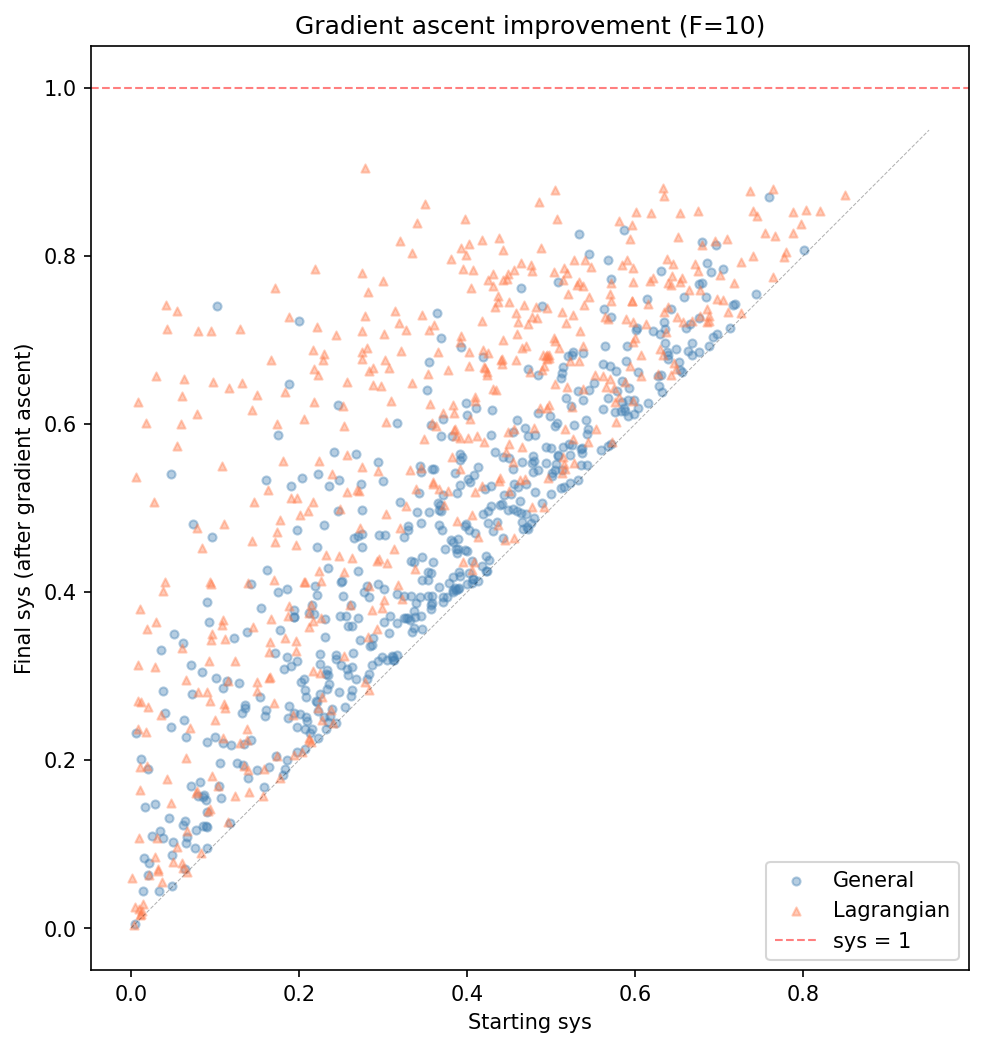
\includegraphics{../experiments/gradient-descent/gradient_descent_scatter.png}
\caption{Starting vs.\ final $\mathrm{sys}$ under gradient ascent.
  Nearly all points lie above the diagonal.
  Lagrangian products (coral) cluster at higher values than
  general polytopes (blue).}
\label{fig:gd-scatter}
\end{figure}

Two patterns are consistent with the known counterexample
of~\cite{HaimKislevOstrover2024} being a $5 \times 5$
Lagrangian product:
Lagrangian products reach higher $\mathrm{sys}$ than general polytopes
(mean~$0.56$ vs.~$0.45$),
and balanced splits outperform asymmetric ones
($5 \times 5$ mean~$0.628$ vs.\ $3 \times 7$ mean~$0.493$).

\subsubsection*{Convergence analysis}

The algorithm terminates with gradient norms bounded away from
zero---far from the near-zero gradients expected at a local maximum.
The median $\|\nabla_h\,\mathrm{sys}\|$ at termination
is~$0.36$ for general polytopes and~$0.53$ for Lagrangian products.
Moreover, $\|\nabla_h\,\mathrm{sys}\|$ is \emph{positively}
correlated with final $\mathrm{sys}$ (Pearson $r \approx 0.80$;
Figure~\ref{fig:gd-gradient}):
polytopes with higher final $\mathrm{sys}$ tend to have
larger residual gradients.

\begin{figure}[htbp]
\centering
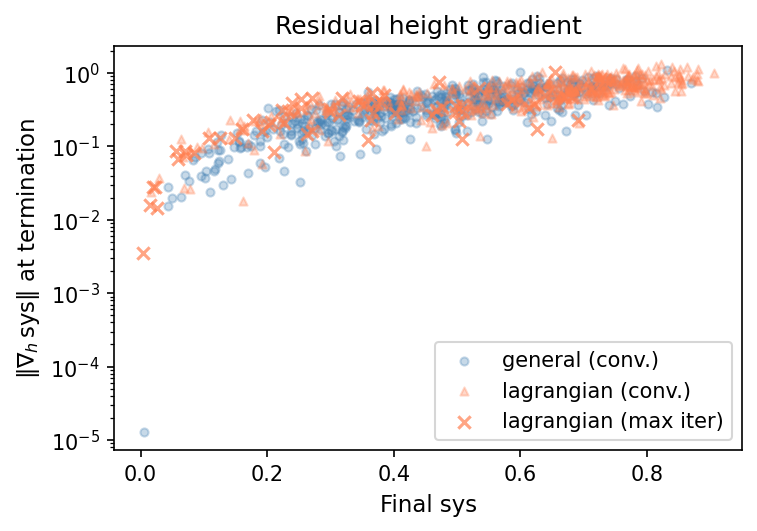
\includegraphics{../experiments/gradient-descent/gradient_descent_gradient.png}
\caption{Residual height gradient $\|\nabla_h\,\mathrm{sys}\|$ vs.\
  final $\mathrm{sys}$ at termination.
  Higher final $\mathrm{sys}$ correlates with
  larger residual gradients ($r \approx 0.80$).}
\label{fig:gd-gradient}
\end{figure}

\begin{figure}[htbp]
\centering
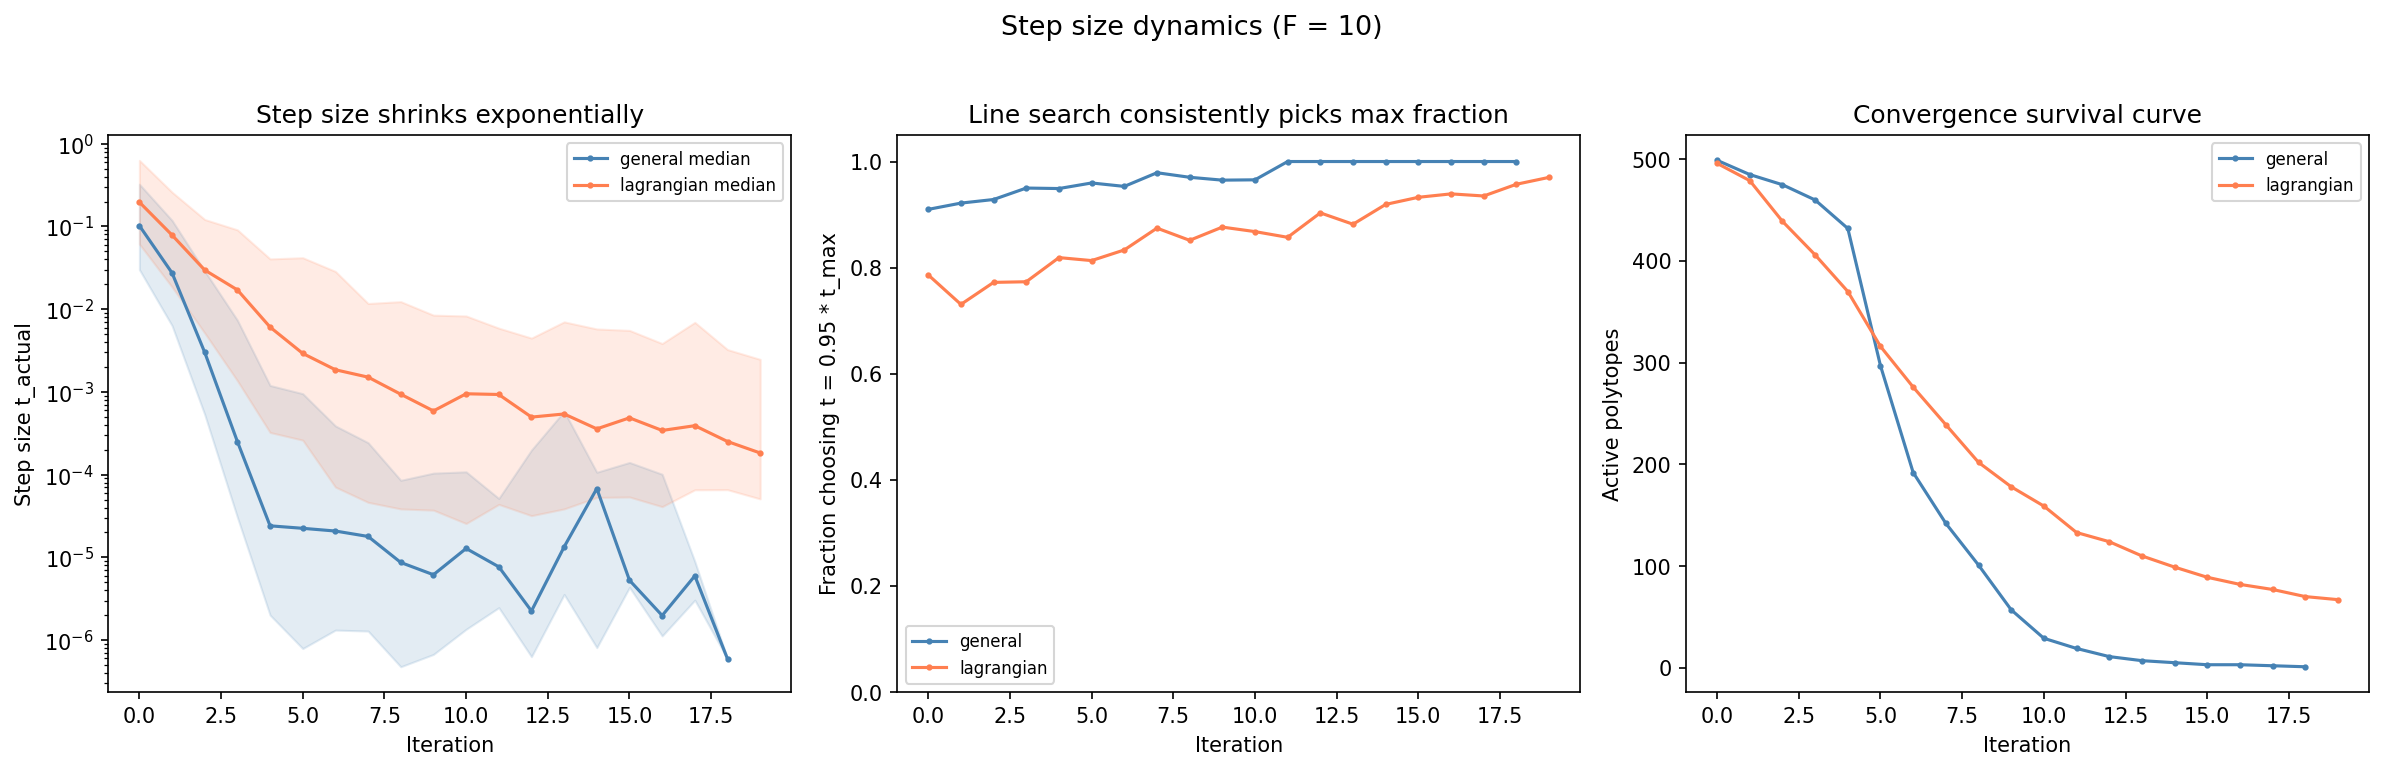
\includegraphics{../experiments/gradient-descent/gradient_descent_stepsize.png}
\caption{Median step size (with IQR band) per iteration.
  The step bound drops by 2--3 orders of magnitude
  over the first 10~iterations.}
\label{fig:gd-stepsize}
\end{figure}

\begin{figure}[htbp]
\centering
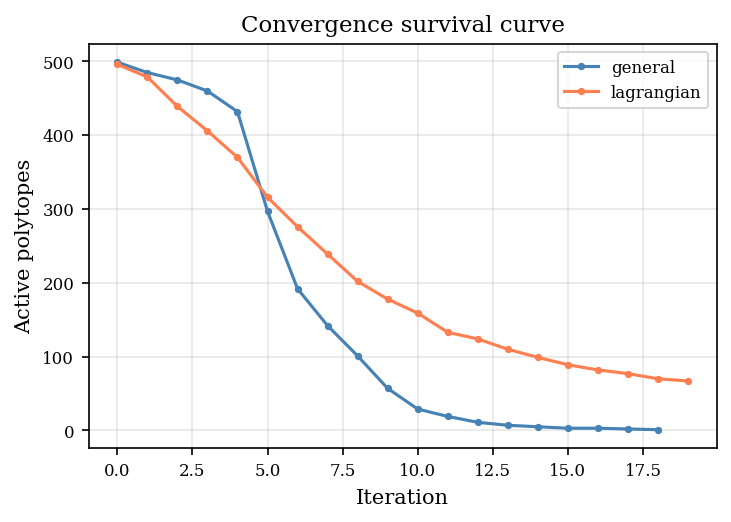
\includegraphics{../experiments/gradient-descent/gradient_descent_survival.png}
\caption{Convergence survival curve: number of polytopes
  still improving at each iteration.}
\label{fig:gd-survival}
\end{figure}

The cause is visible in the step size dynamics
(Figure~\ref{fig:gd-stepsize}):
the step bound~$t_{\max}$ shrinks exponentially,
dropping by 2--3 orders of magnitude over the first 10~iterations.
The line search selects the most aggressive fraction
($0.95 \cdot t_{\max}$) in 87\% of iterations.
In most iterations the algorithm would benefit from a larger step,
but the combinatorial type boundary closes in,
leaving less and less room for improvement.

\subsubsection*{Interpretation}
% [TODO: JÖRN - review interpretation below, especially the claims about
%  basin-of-attraction measure and regular pentagon structure.]

The data is consistent with a \emph{step-bound barrier}
rather than a gradient obstruction:
the algorithm terminates because the step bound shrinks,
not because gradients vanish.
Several factors may contribute to the gap between
$\mathrm{sys} \approx 0.905$ and the threshold~$1$:
\begin{itemize}
\item The combinatorial-type-preserving step bound confines each step
  to the current polytope's cell in parameter space.
  Crossing into a new combinatorial type requires restarting.
\item If a basin of attraction for $\mathrm{sys} > 1$ exists at
  $F = 10$, it may have small measure among random starting points.
\item The counterexample of~\cite{HaimKislevOstrover2024} uses a regular
  pentagon with specific geometric structure; it is unclear whether
  random polygon pairs can approximate this structure.
\end{itemize}
